% Adaptive (covariance) random-walk Metropolis for the 1D shock tube:
% infer the 4 boundary params m = (p_high, p_low, rho_high, rho_low) from
% final-time density observations, with the Euler / exact-Sod forward model.
% Structure mirrors the "Adaptive Transport Map MCMC" reference figure, but the
% transport map is replaced by our actual likelihood + adaptive-covariance kernel.
\documentclass[border=8pt]{standalone}
\usepackage{tikz}
\usepackage{amsmath,amssymb}
\usetikzlibrary{arrows.meta,positioning,fit,backgrounds,calc}

\begin{document}
\begin{tikzpicture}[
  font=\small,
  >={Stealth[length=2.6mm]},
  defbox/.style   = {draw=black, line width=0.8pt, fill=white,
                     inner sep=5pt, align=center},
  bigbox/.style   = {draw=black, line width=0.9pt, fill=white,
                     inner sep=7pt, align=center},
  procbox/.style  = {draw=black, line width=0.9pt, fill=blue!12,
                     inner sep=6pt, align=center, text width=46mm},
  plainbox/.style = {draw=black, line width=0.9pt, fill=white,
                     inner sep=6pt, align=center},
  rejbox/.style   = {draw=black, line width=0.9pt, fill=red!28,
                     inner sep=5pt, align=center},
  accbox/.style   = {draw=black, line width=0.9pt, fill=green!30,
                     inner sep=5pt, align=center},
  flow/.style     = {-{Stealth[length=2.6mm]}, line width=0.9pt},
]

% =====================================================================
% ===  DEFINE  ========================================================
% =====================================================================
\node[font=\bfseries\large] (deftitle) at (0,0) {Define};

% --- Target: posterior over the 4 params -----------------------------
\node[defbox, below left=6mm and 8mm of deftitle] (target) {
  Target: \ $\pi(\mathbf{m}\mid \mathbf{y}^\circ)$\\[2pt]
  {\footnotesize $\mathbf{m}=(p_{\mathrm{hi}},p_{\mathrm{lo}},
                   \rho_{\mathrm{hi}},\rho_{\mathrm{lo}})$}\\[3pt]
  \begin{tikzpicture}[baseline]
    \draw[gray] (-2.1,0) -- (2.1,0);
    \draw[blue, line width=1pt, smooth, samples=60, domain=-2:2]
      plot (\x, {0.62*exp(-2*(\x+0.55)^2) + 0.9*exp(-2.2*(\x-0.5)^2)});
  \end{tikzpicture}};

% --- Proposal: adaptive random-walk kernel ---------------------------
\node[defbox, below right=6mm and 8mm of deftitle] (proposal) {
  Proposal: \ $q\!\left(\cdot \mid \mathbf{m}^{(k)}\right)
              = \mathcal{N}\!\left(\mathbf{m}^{(k)},\, s^2\,C\right)$\\[3pt]
  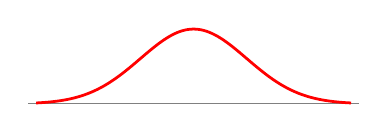
\begin{tikzpicture}[baseline]
    \draw[gray] (-2.1,0) -- (2.1,0);
    \draw[red, line width=1pt, smooth, samples=60, domain=-2:2]
      plot (\x, {0.95*exp(-1.1*\x*\x)});
  \end{tikzpicture}};

% --- Construct: likelihood / forward model / prior -------------------
\node[bigbox, below=44mm of deftitle, text width=104mm] (construct) {
  \textbf{Construct the posterior}\\[3pt]
  Forward model:\ $\mathbf{g}(\mathbf{m})=\rho\big(x_i,\,t_f;\mathbf{m}\big)$
  at observed cells \ \ (\,\emph{Euler} \,/\, \emph{exact Sod}\,)\\[3pt]
  Observations:\ $\mathbf{y}^\circ=\big\{\rho(x_i,t_f)\big\}_{i\in\mathcal{O}}$
  \ (region interiors, fronts excluded)\\[3pt]
  Likelihood:\ $\mathbf{y}^\circ\mid\mathbf{m}\sim
     \mathcal{N}\!\big(\mathbf{g}(\mathbf{m}),\,\sigma^2 I\big)$
  \qquad Prior:\ $\mathbf{m}\sim\mathrm{Unif}(\text{ensemble box})$\\[4pt]
  $\displaystyle
   \pi(\mathbf{m}\mid\mathbf{y}^\circ)\ \propto\
   \exp\!\Big(-\tfrac{1}{2\sigma^2}\,
   \big\|\mathbf{g}(\mathbf{m})-\mathbf{y}^\circ\big\|^2\Big)\,
   \mathbf{1}_{\text{box}}(\mathbf{m})$};

\draw[flow] (target.south)   -- ($(construct.north)+(-2.2,0)$);
\draw[flow] (proposal.south) -- ($(construct.north)+( 2.2,0)$);

% =====================================================================
% ===  ADAPTIVE-COVARIANCE METROPOLIS MCMC  ===========================
% =====================================================================
\node[font=\bfseries\large, below=8mm of construct] (mctitle)
  {Adaptive-Covariance Metropolis MCMC};

% --- top row: propose -> forward solve -> evaluate -------------------
\node[procbox, below=9mm of mctitle.west, anchor=north east, xshift=10mm]
  (propose) {
  \textbf{Propose} (adaptive random walk)\\[2pt]
  $\mathbf{m}' = \mathbf{m}^{(k)} + s\,L\,\mathbf{z},\quad
   \mathbf{z}\sim\mathcal{N}(0,I)$\\[1pt]
  {\footnotesize $L=\mathrm{chol}(C)$, normalized $[0,1]^4$ space}};

\node[plainbox, right=12mm of propose, text width=34mm] (solve) {
  \textbf{Forward solve}\\[2pt]
  $\mathbf{d}'=\mathbf{g}(\mathbf{m}')$\\[1pt]
  {\footnotesize Euler / exact Sod at $t_f$}};

\node[procbox, right=12mm of solve] (eval) {
  \textbf{Evaluate log-posterior}\\[2pt]
  $\log\pi(\mathbf{m}') =
   -\dfrac{\|\mathbf{d}'-\mathbf{y}^\circ\|^2}{2\sigma^2}
   + \log p(\mathbf{m}')$};

% --- acceptance ------------------------------------------------------
\node[plainbox, below=11mm of eval, text width=52mm] (accept) {
  \textbf{Calculate acceptance}\\[3pt]
  $\alpha=\min\!\left(1,\
   \dfrac{\pi(\mathbf{m}')}{\pi(\mathbf{m}^{(k)})}\right)$\\[2pt]
  {\footnotesize symmetric $q\Rightarrow$ ratio cancels}};

% --- accept / reject -------------------------------------------------
\node[rejbox, left=20mm of accept, yshift=7mm] (reject) {
  Rejected\\[1pt] {\footnotesize $\mathbf{m}^{(k+1)}=\mathbf{m}^{(k)}$}};
\node[accbox, left=20mm of accept, yshift=-9mm] (acceptd) {
  Accepted\\[1pt] {\footnotesize $\mathbf{m}^{(k+1)}=\mathbf{m}'$}};

% --- update ----------------------------------------------------------
\node[plainbox, below=8mm of propose, xshift=-2mm, text width=30mm] (update) {
  \textbf{Update}\\[1pt] $\mathbf{m}^{(k+1)}\!\to\mathbf{m}^{(k)}$};

% --- adapt (optional, during burn-in) --------------------------------
\node[bigbox, below=10mm of acceptd, text width=92mm] (adapt) {
  \textbf{Adapt} \ (burn-in only, optional)\\[3pt]
  $C \leftarrow \mathrm{Cov}\big(\text{chain}\big)\quad\Rightarrow\quad
   L=\mathrm{chol}(C)$
  \qquad
  $s \leftarrow s\,\exp\!\Big(\dfrac{\hat\alpha-0.234}{\sqrt{k}}\Big)$};

% --- flow arrows -----------------------------------------------------
\draw[flow] (propose) -- (solve);
\draw[flow] (solve)   -- (eval);
\draw[flow] (eval)    -- (accept);
\draw[flow] (accept.west) -- (reject.east);
\draw[flow] (accept.west) -- (acceptd.east);
\draw[flow] (reject.west)  -| (propose.south)
  node[pos=0.25, above, font=\footnotesize] {resample};
\draw[flow] (acceptd.west) -- (update.east);
\draw[flow] (update.north) -- (propose.south);
\draw[flow, dashed] (acceptd.south) |- (adapt.west);
\draw[flow, dashed] (adapt.east) -| ($(eval.south)+(0.6,0)$)
  node[pos=0.25, below, font=\footnotesize] {update $C,\,s$};

\end{tikzpicture}
\end{document}
